\input ../talk-header.tex
\title
{Machine Learning}
\subtitle{Features and Modeling}

\begin{document}

\begin{frame}
  \vspace{4mm}
  
  \cimgh{titanic-titles.png}
  \vspace{-3mm}
  \prevwork{Kaggle}
\end{frame}

\begin{frame}
  \cimg{reading-time-1.png}
  \prevwork{Jellybooks}
\end{frame}

\begin{frame}
  \cimg{reading-time-2.png}
  \prevwork{Jellybooks}
\end{frame}

\begin{frame}
  \frametitle{pandas}
  \only<1>{\lstinputlisting{pandas_1.py}}
  \only<2>{\purple{\texttt{Dataframe} has many constructors.  For example,}
    \lstinputlisting{pandas_2.py}
  }
  \only<3>{\purple{Viewing data}
    \lstinputlisting{pandas_3.py}
  }
  \only<4>{\purple{Basic data exploration}
    \lstinputlisting{pandas_4.py}
  }
  \only<5>{\purple{Select a column (series)}
    \lstinputlisting{pandas_5.py}
  }
  \only<6>{\purple{Select a range}
    \lstinputlisting{pandas_6.py}
  }
  \only<7>{\purple{Boolean selection criteria}
    \lstinputlisting{pandas_7.py}
  }
  \only<8>{\purple{Recommended}
    
    \vspace{5mm}
    \url{http://www.gregreda.com/2013/10/26/intro-to-pandas-data-structures/}
  }
\end{frame}

\begin{frame}
  \frametitle{Plotting}
  \only<1>{\purple{Draw a line}
    \lstinputlisting{pyplot_1.py}
    \vspace{-19mm}
    \flushright{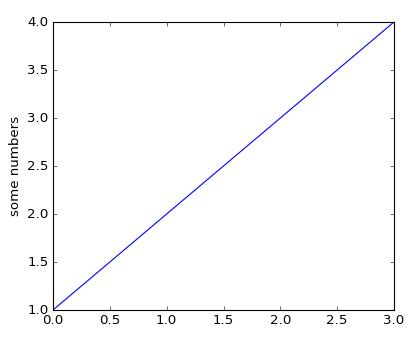
\includegraphics[width=.5\textwidth]{pyplot_1.png}}
  }
  \only<2>{\purple{Draw a line}
    \lstinputlisting{pyplot_2.py}
    \vspace{-19mm}
    \flushright{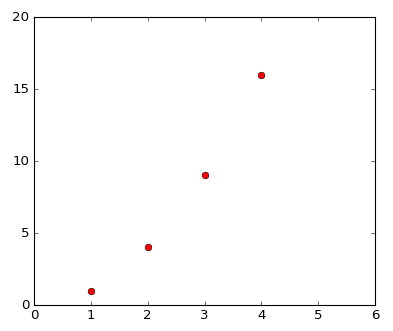
\includegraphics[width=.5\textwidth]{pyplot_2.png}}
  }
  \only<3>{\purple{Draw a line}
    \lstinputlisting{pyplot_3.py}
    \vspace{-55mm}
    \flushright{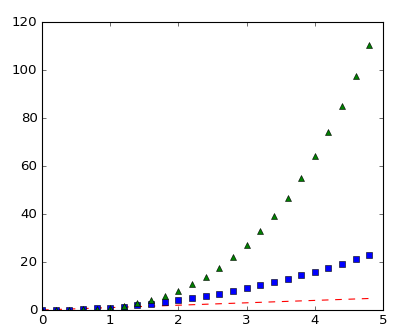
\includegraphics[width=.5\textwidth]{pyplot_3.png}}
  }
  \only<4>{\purple{Draw two curves}
    \lstinputlisting{pyplot_4.py}
  }
  \only<5>{
    \flushright{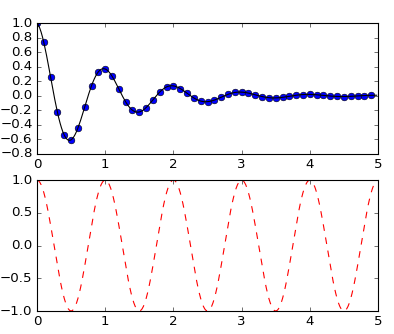
\includegraphics[width=.5\textwidth]{pyplot_4.png}}
  }    
  \only<6>{\purple{Draw two curves}
    \lstinputlisting{pyplot_5.py}
  }
  \only<7>{
    \flushright{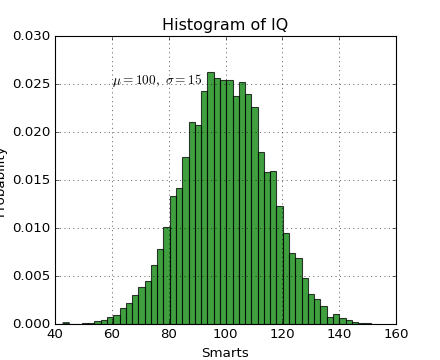
\includegraphics[width=.5\textwidth]{pyplot_5.png}}
  }
  \only<8>{\purple{Scatter plot}
    \prevwork{\url{http://matplotlib.org/mpl_examples/pylab_examples/scatter_demo2.py}}
    \lstinputlisting{pyplot_6.py}
    \vspace{-60mm}
    \flushright{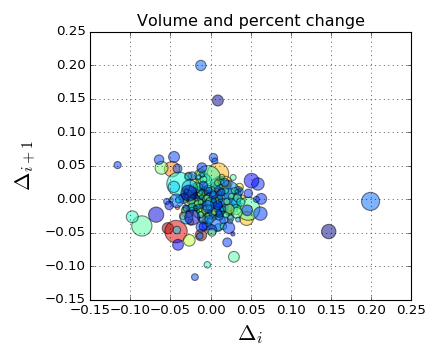
\includegraphics[width=.5\textwidth]{pyplot_6.png}}
    
  }
  \only<9>{
    \prevwork{\url{http://matplotlib.org/users/pyplot_tutorial.html}}
      
    \prevwork{\url{http://matplotlib.org/users/beginner.html}}
  }
\end{frame}

%%%%%%%%%%%%%%%%%%%%%%%%%%%%%% Linear Regression %%%%%%%%%%%%%%%%%%%%%%%%%%%%%%

\begin{frame}
  \frametitle{Linear models}

  \only<1>{
    \textbf{Problem:}  $\{(x_i, y_i)\}$.

    Given $x$, predict $\hat y$.
  }

  \only<2>{ $x$: \textbf{explanatory} or \textbf{predictor} variable.

    $y$: \textbf{response} variable.

    \vspace{1cm}
    \purple{For some reason, we believe a linear model is a good idea.}
  }

  \only<3>{Example:
    \cimgsm{regression-line-1.png}
  }

  \only<4>{Example:
    \cimgsm{regression-line-2.png}
  }

  \only<5>{Example:
    \cimgsm{regression-line-3.png}
  }

  \only<6>{Example:
    \cimg{regression-line-4.png}
  }
\end{frame}

\begin{frame}
  \frametitle{Residuals}

  What's left over.

  \only<1>{
    \vspace{1cm}
    \begin{displaymath}
      \text{data} = \text{fit} + \text{residual}      
    \end{displaymath}
  }
  \only<2>{
    \vspace{1cm}
    \begin{displaymath}
      y_i = \hat y_i + e_i
    \end{displaymath}
  }

  \only<3>{\vfill\cimg{residuals-1.png}}
  \only<4>{\vfill\cimg{residuals-2.png}}
  
  \only<5>{
    Goal: small residuals.

    \vspace{1cm}
    \begin{displaymath}
      \sum \mid e_i\mid
    \end{displaymath}
  }
  \only<6>{
    Goal: small residuals.

    \vspace{1cm}
    \begin{displaymath}
      \sum e_i^2
    \end{displaymath}
  }
\end{frame}

\begin{frame}
  \frametitle{Outliers}

  \only<1>{
    \vfill
    \cimghh{outliers-1.png}
    \cnote{
      There is one outlier far from the other points, though it only
      appears to slightly influence the line.
    }
  }
  
  \only<2>{
    \vfill
    \cimghh{outliers-2.png}
    \cnote{There is one outlier on the right, though it is quite close
      to the least squares line, which suggests it wasn’t very influential.
    }
  }
  
  \only<3>{
    \vfill
    \cimghh{outliers-3.png}
    \cnote{There is one point far away from the cloud, and this outlier appears to pull the
      least squares line up on the right; examine how the line around the primary
      cloud doesn’t appear to fit very well.
    }
  }
  
  \only<4>{
    \vfill
    \cimghh{outliers-4.png}
    \cnote{There is a primary cloud and then a small secondary cloud of four outliers. The
      secondary cloud appears to be influencing the line somewhat strongly, making
      the least square line fit poorly almost everywhere. There might be an interesting
      explanation for the dual clouds, which is something that could be investigated.
    }
  }
  
  \only<5>{
    \vfill
    \cimghh{outliers-5.png}
    \cnote{There is no obvious trend in the main cloud of points and the outlier on the
      right appears to largely control the slope of the least squares line.
    }
  }
  
  \only<6>{
    \vfill
    \cimghh{outliers-6.png}
    \cnote{There is one outlier far from the cloud, however, it falls quite close to the least
      squares line and does not appear to be very influential.
    }
  }

  \only<7>{
    \vfill\centerline{\huge Don't ignore outliers.}
  }

  \only<8>{
    \vfill
    \cimg{outliers-important.png}
  }
\end{frame}

\begin{frame}
  \frametitle{Correlation}

  \only<1>{\vfill\cimgg{correlations-1.png}}
  \only<2>{\vfill\cimg{correlations-2.png}}
  \only<3>{Anscombe's Quartet

    \cimghh{anscombe_quartet.png}
  }
\end{frame}

\begin{frame}
  \vphrase{Correlation does not imply causation}
\end{frame}

\begin{frame}
  \frametitle{Hypothesis (model)}
  \begin{mphrase}
    h_\theta(x) = \theta_0 + \theta_1 x
  \end{mphrase}
\end{frame}

\begin{frame}
  \frametitle{Cost function}
  \begin{mphrase}
    J(\theta_0, \theta_1) = \frac{1}{2m} \sum_{i=1}^m (h_\theta(x_i) - y_i)^2
  \end{mphrase}
\end{frame}

\begin{frame}
  \frametitle{Gradient descent}

  \begin{mphrase}
      \begin{dcases}
        \theta_0 & \leftarrow\, \theta_0 - \alpha
        \frac{\partial}{\partial\theta_0}\, J(\theta_0, \theta_1)\\[2mm]
%
        \theta_1 & \leftarrow\, \theta_1 - \alpha
        \frac{\partial}{\partial\theta_1}\, J(\theta_0, \theta_1)
      \end{dcases}
  \end{mphrase}
\end{frame}

\begin{frame}
  \frametitle{Gradient descent}

  \begin{mphrase}
    \begin{dcases}
      \theta_0 & \leftarrow \, \theta_0 - 
                 \frac{\alpha}{m} \sum_{i=1}^m (h_\theta(x_i) - y_i)
                 \\[2mm]
%
      \theta_1 & \leftarrow \, \theta_1 -
                 \frac{\alpha}{m} \sum_{i=1}^m (h_\theta(x_i) - y_i)
    \end{dcases}
  \end{mphrase}
\end{frame}

\begin{frame}
  \cimgh{parameter-space.png}
\end{frame}

\begin{frame}
  \frametitle{Hypothesis again}

  \begin{bphrase}
    \begin{align*}
      h_\theta(x) & = \theta_0 + \theta_1 x_1 \\[2mm]
      & = \theta_0 + \sum_{i=1}^1 \theta_i x_i \\[2mm]
      & = [\theta_0, \theta_1]
        \begin{bmatrix}
          x_0\\ x_1
        \end{bmatrix} \\[2mm]
      & = \theta^T x
    \end{align*}
  \end{bphrase}
\end{frame}

\begin{frame}
  \frametitle{Hypothesis (multiple regression)}

  \begin{bphrase}
    \begin{align*}
      h_\theta(x) & = \theta_0 + \sum_{i=1}^n \theta_i x_i \\[2mm]
      & = [\theta_0, \cdots, \theta_n]
        \begin{bmatrix}
          x_0\\ x_1 \\ \vdots \\ x_n
        \end{bmatrix} \\[2mm]
      & = \theta^T x
    \end{align*}
  \end{bphrase}
\end{frame}

\begin{frame}
  \frametitle{Hypothesis (multiple regression)}

  \begin{bphrase}
    \begin{align*}
      h_\theta(x) & = \theta^T x \\[2mm]
      & = \theta^T x^{(1)}
    \end{align*}
  \end{bphrase}
\end{frame}

\begin{frame}
  \frametitle{Hypothesis (multiple regression)}

  \begin{mphrase}
    X =
    \begin{bmatrix}
      \vline & \vline & \cdots & \vline \\
      x^{(1)} & x^{(2)} & \cdots & x^{(m)} \\
      \vline & \vline & \cdots & \vline \\
    \end{bmatrix} =
    \begin{bmatrix}
      x_0^{(1)} & x_0^{(2)} & \cdots & x_0^{(m)} \\[2mm]
      x_1^{(1)} & x_1^{(2)} & \cdots & x_1^{(m)} \\
      \vdots & \vdots & \ddots & \vdots \\
      x_n^{(1)} & x_n^{(2)} & \cdots & x_n^{(m)} \\
    \end{bmatrix}
  \end{mphrase}
\end{frame}

\begin{frame}
  \frametitle{Hypothesis (multiple regression)}

  \begin{bphrase}
    \begin{align*}
      h_\theta(X) & = \theta^T X \\[2mm]
      & =
        \begin{bmatrix}
          h_0(x^{(1)}), h_0(x^{(2)}), \cdots, h_0(x^{(m)})
        \end{bmatrix} \\
                  & = \theta^T X
    \end{align*}
  \end{bphrase}
\end{frame}

\begin{frame}
  \frametitle{Hypothesis (multiple regression)}

  \sphrase{or $X\theta$ if row vectors\ldots}
\end{frame}

\begin{frame}
  \frametitle{Cost function (multiple regression)}

  \begin{bphrase}
    \begin{align*}
      J(\theta) & = \frac{1}{2m} \sum_{i=1}^m
                  \left(h_{\theta}(x^{(i)}) - y^{(i)}\right)^2 \\
      &= \frac{1}{2m} (X\theta - Y)^T (X\theta - Y)
    \end{align*}
  \end{bphrase}
\end{frame}

\begin{frame}
  \frametitle{Gradient descent (multiple regression)}

  \begin{bphrase}
    \begin{align*}
      \theta_j & \leftarrow\, \theta_j - \frac{\alpha}{m} \sum_{i=1}^m
                 \left(h_{\theta}(x^{(i)}) - y^{(i)}\right) \cdot x_j^{(i)} \\
    \end{align*}
    \centerline{for $j=1, \cdots, n$}
  \end{bphrase}
\end{frame}

\begin{frame}
  \frametitle{Gradient descent (multiple regression)}

  \begin{bphrase}
    \begin{align*}
      \theta & \leftarrow\, \theta - \nabla J(\theta)
    \end{align*}

    \begin{displaymath}
      \mbox{where } \nabla =
      \begin{bmatrix}
        \frac{\partial}{\partial\theta_0} \\[2mm]
        \frac{\partial}{\partial\theta_1} \\[2mm]
        \vdots\\[2mm]
        \frac{\partial}{\partial\theta_n} \\
      \end{bmatrix}
    \end{displaymath}
  \end{bphrase}
\end{frame}


\end{document}
